\section{Calculo de Esperança, Variância e Lei dos Grandes Números}
Esta seção aborda a validação empírica dos conceitos de Esperança Matemática ($E[X]$) e Variância ($\Var(X)$), estendendo a análise para a verificação do fenômeno da estabilidade estatística ditado pela Lei dos Grandes Números (LGN).

\subsection{Definições Teóricas}

A Lei dos Grandes Números garante que a média amostral de ensaios independentes converge para a média teórica populacional quando o número de ensaios tende ao infinito:
\begin{equation}
    P\left( \lim_{k \to \infty} \bar{X}_k = \mu \right) = 1
\end{equation}

Utilizou-se uma variável aleatória contínua $X \sim Exp(\lambda = 0.2)$. Os parâmetros teóricos de controle de longa duração são definidos matematicamente por:
\begin{align}
    E[X] &= \frac{1}{\lambda} = \frac{1}{0.2} = 5.0000 \\
    \Var(X) &= \frac{1}{\lambda^2} = \frac{1}{0.04} = 25.0000
\end{align}

\subsection{Resultados e Análise Crítica}

Após a execução da simulação computacional para $K = 10.000$ ensaios independentes, os valores empíricos organizados comparativamente são apresentados na Tabela \ref{tab:t4_comparativo}.

\begin{table}[H]
    \centering
    \caption{Comparação entre Parâmetros Teóricos e Estimativas Empíricas ($K=10.000$).}
    \label{tab:t4_comparativo}
    \vspace{2mm}
    \begin{tabular}{lccc}
        \toprule
        \textbf{Métrica} & \textbf{Valor Teórico} & \textbf{Estimativa Empírica} & \textbf{Erro Relativo (\%)} \\ \midrule
        Esperança $E[X]$ & 5,0000 & 5,0189 & 0,38\% \\
        Variância $\Var(X)$ & 25,0000 & 24,9941 & 0,02\% \\ \bottomrule
    \end{tabular}
\end{table}

A visualização do processo dinâmico de convergência da média móvel ao longo das iterações é apresentada na Figura \ref{fig:t4_grafico}.

\begin{figure}[H]
    \centering
    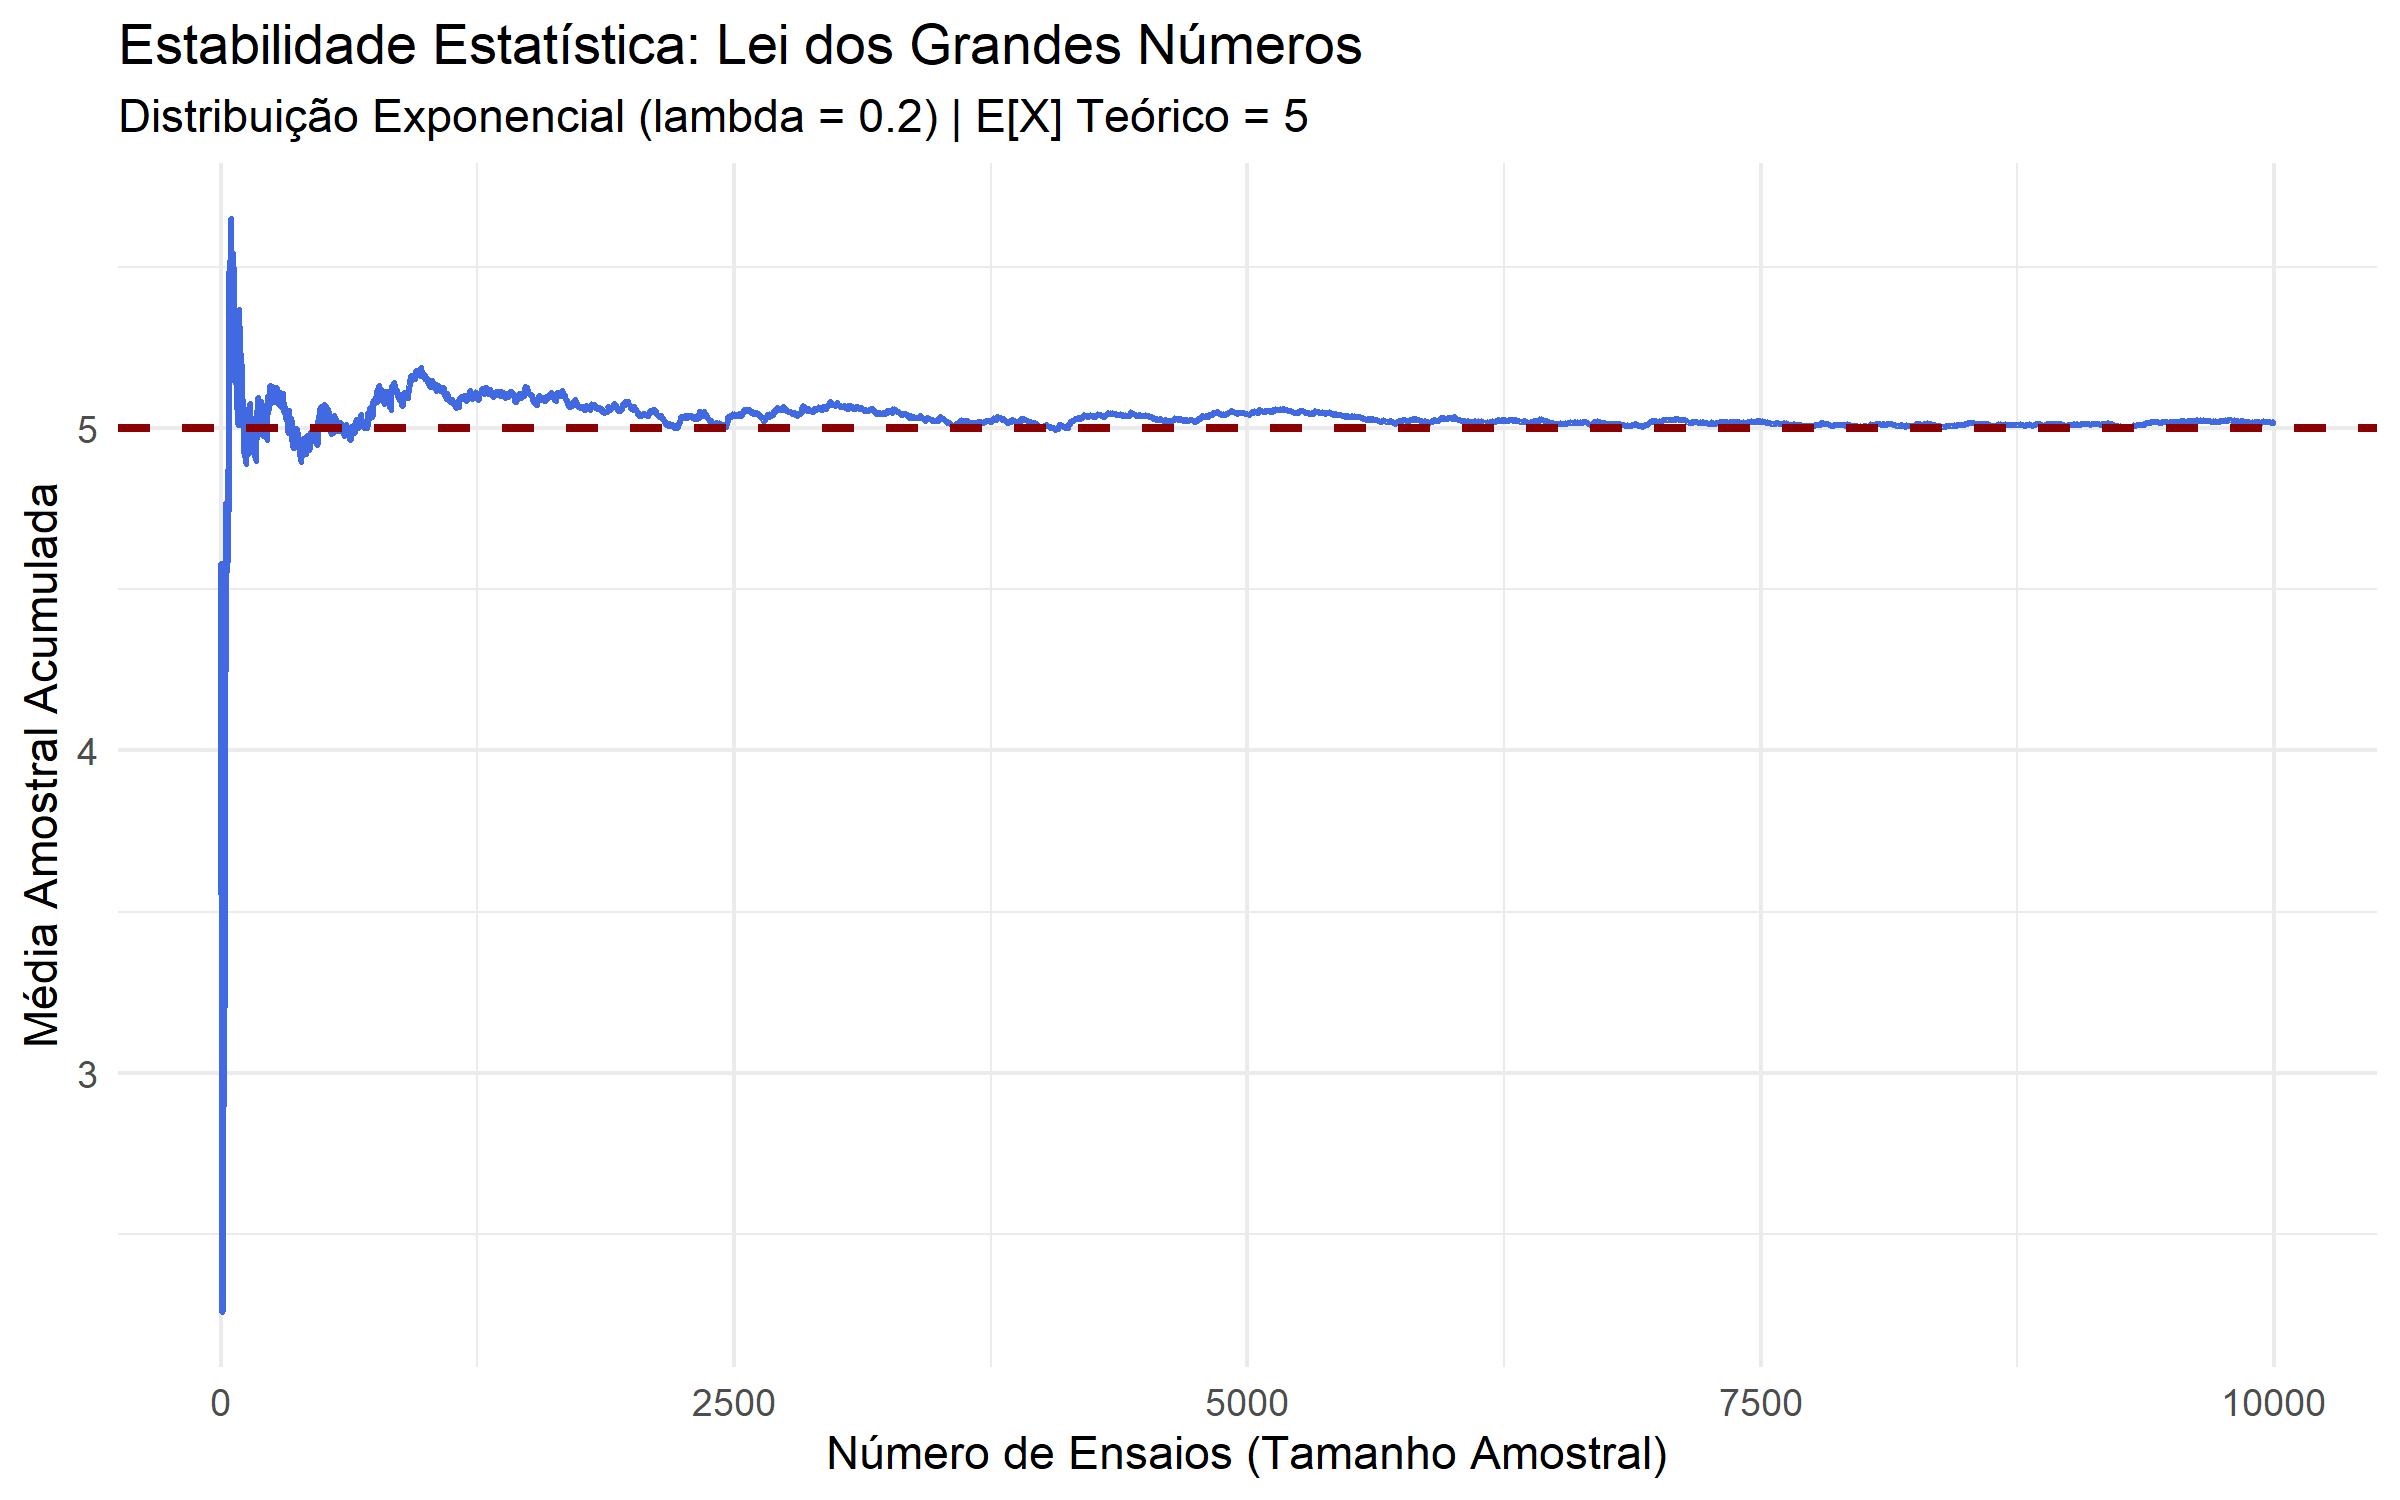
\includegraphics[width=0.85\textwidth]{imagens/t4_lei_grandes_numeros.png}
    \caption{Evolução da média amostral acumulada em função do número de ensaios, demonstrando a convergência assintótica para a expectativa teórica.}
    \label{fig:t4_grafico}
\end{figure}

A interpretação do comportamento da curva permite extrair conclusões científicas sobre a estabilidade estatística:
\begin{itemize}
    \item \textbf{Flutuações Iniciais (Baixo $K$):} Nos primeiros ensaios, a variabilidade do estimador é agressiva. Como a variância da distribuição original é alta ($\Var(X) = 25$), a ocorrência de valores extremos desloca bruscamente a linha da média móvel.
    \item \textbf{Amortecimento:} À medida que o tamanho amostral cresce, o efeito de novos sorteios individuais isolados passa a ser diluído pelo denominador crescente da média móvel.
    \item \textbf{Convergência:} Próximo a $K = 10.000$, as oscilações tornam-se imperceptíveis, tangenciando a linha teórica. O baixíssimo erro relativo obtido valida o funcionamento das simulações computacionais estocásticas.
\end{itemize}

O código-fonte utilizado para esta análise encontra-se disponível no Código \ref{lst:script_t4}.

\begin{lstlisting}[language=R, caption={Validação da Lei dos Grandes Números (T4).}, label=lst:script_t4]
# T4: Esperança, Variância e Lei dos Grandes Números
set.seed(123)

if(!require(ggplot2)) install.packages("ggplot2")
library(ggplot2)

lambda <- 0.2
K <- 10000
mu_teorica <- 1 / lambda

amostras <- rexp(K, rate = lambda)
medias_acumuladas <- cumsum(amostras) / (1:K)

df_lgn <- data.frame(Ensaio = 1:K, Media_Acumulada = medias_acumuladas)

p_lgn <- ggplot(df_lgn, aes(x = Ensaio, y = Media_Acumulada)) +
  geom_line(color = "royalblue", linewidth = 0.7) +
  geom_hline(yintercept = mu_teorica, color = "darkred", linetype = "dashed", linewidth = 1) +
  labs(title = "Estabilidade Estatística: Lei dos Grandes Números",
       x = "Número de Ensaios (Tamanho Amostral)",
       y = "Média Amostral Acumulada") +
  theme_minimal()

ggsave("imagens/t4_lei_grandes_numeros.png", p_lgn, width = 8, height = 5)
\end{lstlisting}
